\documentclass[pra,12pt]{revtex4}
\usepackage{amsmath}
\usepackage{amssymb}
\usepackage{graphicx}
\usepackage{color}
\usepackage[pdfborder={0 0 0},colorlinks=true,linkcolor=blue,urlcolor=blue]{hyperref}

\def\ket#1{\left|#1\right\rangle}
\def\bra#1{\left\langle#1\right|}
\def\braket#1{\left\langle#1\right\rangle}

\setlength{\parindent}{0pt}

\renewcommand{\baselinestretch}{1.0}
\setlength{\parskip}{0.07in}

\begin{document}

\section*{Appendix B: The Transfer Matrix Method}

The \textbf{transfer matrix method} is a numerical method for solving
the 1D Schr\"odinger equation, and other similar equations.  In this
method, the wavefunction at each point is decomposed into two complex
numbers, called wave components.  The wave components at any two
points are related by a complex $2\times2$ matrix, called the
\textbf{transfer matrix}.

\section{Wave components in 1D}

For a 1D space with spatial coordinates $x$, the Schr\"odinger wave
equation is
$$-\frac{\hbar^2}{2m}\frac{d^2\psi}{dx^2} + V(x) \psi(x) = E\psi(x),$$
where $m$ is the particle mass, $\psi(x)$ is the wavefunction, $V(x)$
is the potential function, and $E$ is the energy.  We treat $E$ as an
adjustable parameter (e.g., the energy of the incident particle in a
scattering experiment).

Within any region of space where $V$ is constant, the Schr\"odinger
equation reduces to a 1D Helmholtz equation, whose general solution is
$$\psi(x) = A\, e^{ik x} + B\, e^{-ik x}, \;\;\; \mathrm{where}\;\; k = \sqrt{\frac{2m[E-V(x)]}{\hbar^2}}.$$
If $E > V$, then the wave-number $k$ is real and positive, and
$\exp(\pm ikx)$ denotes a right-moving ($+$) or left-moving ($-$)
wave.  If $E < V$, then $k$ is purely imaginary, and we choose the
branch of the square root so that it is a positive multiple of $i$, so
that $\exp(\pm ikx)$ denotes a wave that \textit{decreases}
exponentially toward the right ($+$) or toward the left ($-$).

We can re-write the two terms on the right-hand side as
$$\psi(x) = \psi_+(x) + \psi_-(x).$$
At each position $x$, the complex quantities $\psi_\pm(x)$ are called
the \textbf{wave components} .

The problem statement for the transfer matrix method is as follows.
Suppose we have a \textbf{piecewise-constant potential function}
$V(x)$, which takes on values $\{V_1, V_2, V_3, \dots\}$ in different
regions of space, as shown in the figure below:

\begin{center}
  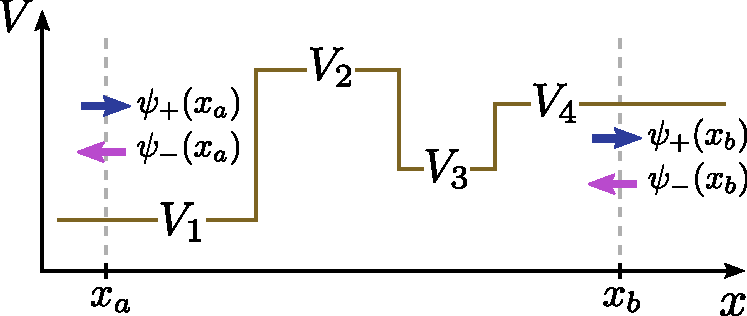
\includegraphics[width=0.45\textwidth]{transfer_matrix_setup}
\end{center}

Given the wave components $\{\psi_+(x_a),\psi_-(x_a)\}$ at one
position $x_a$, we seek to compute the wave components
$\{\psi_+(x_b),\psi_-(x_b)\}$ at another position $x_b$.  In general,
these are related by a linear relation
$$\Psi_b = \mathbf{M}(x_b,x_a) \, \Psi_a,$$
where
$$\Psi_b = \begin{bmatrix}\psi_+(x_b) \\ \psi_-(x_b)\end{bmatrix}, \; \Psi_a = \begin{bmatrix}\psi_+(x_a) \\ \psi_-(x_a)\end{bmatrix}.$$
The $2\times2$ matrix $\mathbf{M}(x_b,x_a)$ is called a
\textbf{transfer matrix}.  Take note of the notation in the
parentheses: we put the ``start point'' $x_a$ in the right-hand input,
and the ``end point'' $x_b$ in the left-hand input.  We want to find
$\mathbf{M}(x_b,x_a)$ from the potential and the energy $E$.

\section{Constructing the transfer matrix}

\subsection{Transfer matrix across a uniform region}

Consider the simplest possible case, where the potential has a single
constant value $V$ everywhere between two positions $x_a$ and $x_b$,
with $x_b > x_a$.  Then, as we have just discussed, the solution
throughout this region takes the form
$$\psi(x) = A e^{ik x} + B e^{-ik x}, \;\;\; \mathrm{where}\;\; k = \sqrt{\frac{2m(E-V)}{\hbar^2}},$$
for some $A, B\in\mathbb{C}$.  The wave components at the two
positions are
$$\Psi_a = \begin{bmatrix} A e^{ik x_a} \\ B e^{ikx_a} \end{bmatrix}, \;\; \Psi_b = \begin{bmatrix} A e^{ik x_b} \\ B e^{ikx_b} \end{bmatrix}.$$
Each component of $\Psi_b$ is $\exp[ik(x_b-x_a)]$ times the
corresponding component of $\Psi_a$.  We can therefore eliminate $A$
and $B$, and write
$$\Psi_b = \mathbf{M}_0(k, x_b-x_a) \Psi_a, \;\;\;\mathrm{where}\;\;\; \mathbf{M}_0(k,L) \equiv \begin{bmatrix}e^{ikL} & 0 \\ 0 & e^{-ikL}\end{bmatrix}.$$
The $2\times2$ matrix $\mathbf{M}_0(k,L)$ is the transfer matrix
across a segment of constant potential.  Its first input is the
wave-number within the segment (determined by the energy $E$ and
potential $V$), and its second input is the segment length.

\subsection{Transfer matrix across a potential step}

Next, consider a potential step occurring at some position $x_0$, as
shown in the figure below:

\begin{center}
  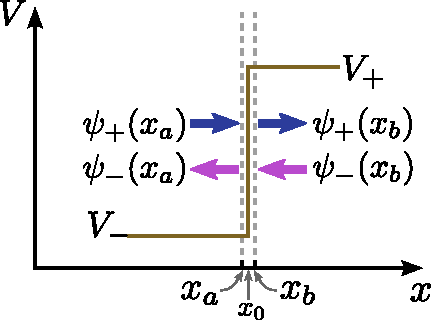
\includegraphics[width=0.32\textwidth]{transfer_step}
\end{center}

Let $x_a$ and $x_b$ be two points that are infinitesimally close to
the potential step on either side (i.e., $x_a = x_0 - 0^+$ and $x_b =
x_0 + 0^+$, where $0^+$ denotes a positive infinitesimal).  To the
left of the step, the potential is $V_-$; to the right, the potential
is $V_+$.  The corresponding wave-numbers are
$$k_\pm = \sqrt{\frac{2m(E-V_\pm)}{\hbar^2}}.$$

There are two important relations between the wavefunctions on the two
sides of the step.  Firstly, any quantum mechanical wavefunction must
be continuous everywhere (otherwise, the Schr\"odinger equation would
not be well-defined); this includes the point $x_0$, so
$$\psi_+(x_a) + \psi_-(x_a) = \psi_+(x_b) + \psi_-(x_b).$$

Secondly, since the potential is non-singular at $x_0$ the derivative
of the wavefunction should be continuous at that point (this can be
shown formally by integrating the Schr\"odinger across an
infinitesimal interval around $x_0$).  Hence,
$$ik_-\, \left[\psi_+(x_a) - \psi_-(x_a)\right] = ik_+\, \left[\psi_+(x_b) - \psi_-(x_b)\right].$$
These two equations can be combined into a single matrix equation:
$$\begin{bmatrix}1 & 1 \\ k_- & - k_-\end{bmatrix}\begin{bmatrix}\psi_+(x_a) \\ \psi_-(x_a) \end{bmatrix} = \begin{bmatrix}1 & 1 \\ k_+ & - k_+\end{bmatrix} \begin{bmatrix}\psi_+(x_b) \\ \psi_-(x_b) \end{bmatrix}.$$
After doing a matrix inversion, this becomes
$$\Psi_b = \mathbf{M}_s(k_+,k_-) \, \Psi_a, \;\;\;\mathrm{where}\;\; \mathbf{M}_s(k_+,k_-) = \frac{1}{2} \begin{bmatrix}1+\frac{k_-}{k_+} & 1-\frac{k_-}{k_+} \\ 1-\frac{k_-}{k_+} & 1+\frac{k_-}{k_+}\end{bmatrix}.$$
The $2\times2$ matrix $\mathbf{M}_s(k_+,k_-)$ is the transfer matrix
to go rightward from a region of wave-number $k_-$, to a region of
wave-number $k_+$.  Note that when $k_- = k_+$, this reduces to the
identity matrix, as expected.

\subsection{Transfer matrix across a piecewise-constant system}

Using the results of the previous two sections, we can find the
transfer matrix for any piecewise-constant potential.  Consider the
potential function shown below.  It consists of segments of length
$L_1, L_2, \dots L_N$, with potential $V_1, V_2, \dots, V_N$; outside,
the potential is $V_0$:

\begin{center}
  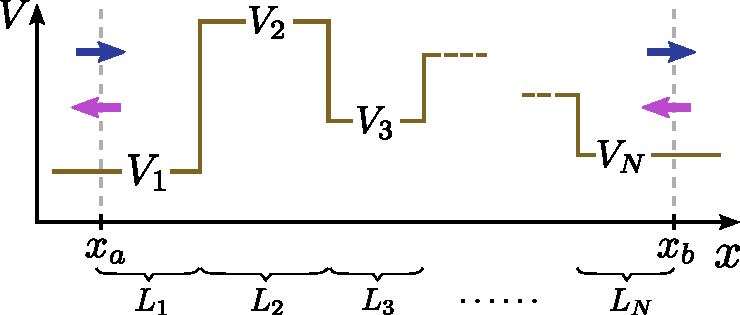
\includegraphics[width=0.5\textwidth]{transfer_matrix_setup2}
\end{center}

Let $x_a$ and $x_b$ lie right beyond the first and last segments
(where $V = V_0$), with $x_b > x_a$.  We can compute $\Psi_b$ by
starting with $\Psi_a$, and left-multiplying by a sequence of transfer
matrices, one after the other.  These transfer matrices consist of the
two types derived in the previous sections: $\mathbf{M}_0$ (to cross a
uniform segment) and $\mathbf{M}_s$ (to cross a potential step).  Each
matrix multiplication ``transfers'' us to another point to the right,
until we reach $x_b$.

Therefore, the overall transfer matrix between the two points is
$$\boxed{\;\;\;\begin{aligned}\mathbf{M}(x_b, x_a) &= \mathbf{M}_s(k_0,k_N)\; \mathbf{M}_0(k_N,L_N) \; \mathbf{M}_s(k_N, k_{N-1}) \cdots \\ & \quad\;\cdots \times \mathbf{M}_s(k_3, k_2)\; \mathbf{M}_0(k_2,L_2) \; \mathbf{M}_s(k_2, k_1) \; \mathbf{M}_0(k_1,L_1) \; \mathbf{M}_s(k_1,k_0) \;\;\;\\ \mathrm{where}\;\;\; \mathbf{M}_0(k,L) &= \begin{bmatrix}e^{ikL} & 0 \\ 0 & e^{-ikL}\end{bmatrix} \\ \mathbf{M}_s(k_+,k_-) &= \frac{1}{2} \begin{bmatrix}1+\frac{k_-}{k_+} & 1-\frac{k_-}{k_+} \\ 1-\frac{k_-}{k_+} & 1+\frac{k_-}{k_+}\end{bmatrix}\\ k_n &= \sqrt{\frac{2m(E-V_n)}{\hbar^2}}.\end{aligned}}$$
The expression for $\mathbf{M}(x_b,x_a)$ should be read from right to
left.  Starting from $x_a$, we cross the potential step into segment
1, then pass through segment 1, cross the potential step from segment
1 to segment 2, pass through segment 2, and so forth.  (Note that as
we move left-to-right through the structure, the matrices are
assembled right-to-left; a common mistake when writing a program to
implement the transfer matrix method is to assemble the matrices in
the wrong order, i.e.~right-multiplying instead of left-multiplying.)

\section{Reflection and transmission coefficients}

The transfer matrix method is typically used to study how a 1D
potential scatters an incident wave.  Consider a 1D scatterer that is
confined within a region $x_a \le x \le x_b$:
$$V(x) = 0 \;\;\;\mathrm{for}\;\;x < x_a \;\textrm{or}\; x > x_b.$$
The total wavefunction consists of an incident wave and a scattered
wave,
$$\psi(x) = \psi_i(x) + \psi_s(x).$$
The incident wave is assumed to be incident from the left:
$$\psi_i(x) = \Psi_i \, \exp[ik_0(x-x_a)], \;\;\;\textrm{where}\;\;\; k_0 = \sqrt{\frac{2mE}{\hbar^2}}.$$
We have inserted the extra phase factor of $\exp(-ik_0x_a)$ to ensure
that $\psi_i(x_a) = \Psi_i$, which will be convenient.  The wave is
scattered as it meets the structure, and part of it is reflected back
to the left, while another part is transmitted across to the right.
Due to the linearity of the Schr\"odinger wave equation, the total
wavefunction must be directly proportional to $\Psi_i$.  Let us
write the wave components at $x_z$ and $x_b$ as
$$\begin{aligned} \Psi(x_a) &= \begin{bmatrix}\psi_+(x_a) \\ \psi_-(x_a) \end{bmatrix} = \Psi_i \begin{bmatrix}\,\,1\, \\ r \end{bmatrix} \\ \Psi(x_b) &= \begin{bmatrix}\psi_+(x_b) \\ \psi_-(x_b) \end{bmatrix} = \Psi_i \begin{bmatrix}\,\,t\,\, \\ 0 \end{bmatrix}.\end{aligned}$$
The complex numbers $r$ and $t$ are called the \textbf{reflection
  coefficient} and the \textbf{transmission coefficient},
respectively.  Their values do \textit{not} depend on $\Psi_i$, since
they specify the wave components for the reflected and transmitted
waves \textit{relative} to $\Psi_i$.  Note also that there is no
$\psi_-$ wave component at $x_b$, as the scattered wavefunction
must be purely outgoing.

\begin{center}
  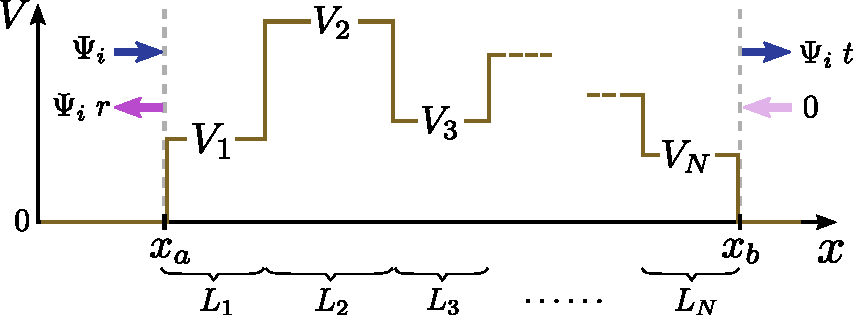
\includegraphics[width=0.65\textwidth]{transfer_matrix_setup3}
\end{center}

From the reflection and transmisison coefficients, we can also define
the real quantities
$$R = |r|^2, \;\;\; T = |t|^2,$$
which are called the \textbf{reflectance} and \textbf{transmittance}
respectively.  These are directly proportional to the total current
flowing to the left and right.

According to the transfer matrix relation,
$$\begin{bmatrix}\,t\, \\ 0 \end{bmatrix} = \textbf{M}(x_b,x_a) \begin{bmatrix}\,1\, \\ r
\end{bmatrix}.$$
Hence, $r$ and $t$ can be expressed in terms of the components of the
transfer matrix:
$$r = \frac{M_{21}}{M_{22}}, \quad t = \frac{M_{11} M_{22} - M_{12}M_{21}}{M_{22}} = \frac{\det(\textbf{M})}{M_{22}}.$$

\end{document}


When $n(x)$ is everywhere real, the reflectance and transmittance obey the equation

: $R + T = 1.$

The squared amplitude of a traveling wave can be interpreted as its "intensity": a quantity that describes the rate at which energy is transported along by the wave.  Thus, $R$ and $T$ correspond to the intensities of the reflected and transmitted waves, normalized to the intensity of the incident wave.  The fact that they sum up to one is thus a statement of the conservation of energy.

The conservation equation can be derived from the wave equation.  [[Energy conservation in 1D wave equation|See this page for the proof.]]

==== Example: scattering from a uniform block ====

As a simple but instructive example of wave scattering, consider a uniform block of refractive index $n_1$ and length $L$.  The refractive index function is

: $n(x) = \left\{\begin{array}{ll}n_1, & 0 \le x \le L,\\ 1 & \mathrm{otherwise}. \end{array}\right.$

In the context of wave scattering, this kind of uniform block structure is called an "etalon", a French word meaning "standard” (because it is the simplest example of a non-trivial scatterer).

It suffices to place the measurement points $x_a$ and $x_b$ infinitesimally to the left and right of the etalon, respectively.  Then, according to the formula we have developed [[#Transfer matrix across a piecewise-constant system|above]], the transfer matrix is

: $\mathbf{M} = \mathbf{Q}(1,n_1)\,\mathbf{P}(n_1,L)\,\mathbf{Q}(n_1,1).$

The transfer matrix also depends on the frequency $\omega$, which enters in the sub-matrix $\mathbf{P}$.  Further examination reveals that the etalon's transfer matrix has a special property: it depends on $\omega$ and $L$ only via the combination $\omega L$.

We can compute the transfer matrix numerically, and hence obtain the reflectance and transmittance.  The results are shown in Fig. 4.  The reflectance and transmittance are plotted against $\omega L$, which we could either think of as varying $L$ while keeping $\omega$ fixed, or vice versa.  Also plotted are the complex arguments of the reflection and transmission coefficients.  These quantities are physically meaningful too; they reveal how the phase of the reflected or transmitted wave changes as we vary the scatterer length $L$, keeping the wave frequency $\omega$ fixed.

[[File:Etalon rt.svg|frame|center|upright|Fig. 4: Reflectance and transmittance (upper plots), and the complex arguments of the reflection and transmission coefficients (lower plots), versus $\omega L$, for uniform blocks of refractive index $n_1=3$ and $n_1=10$.]]

The scattering behavior of the etalon exhibits several interesting features:

* For $\omega L \rightarrow 0$, the wave is completely transmitted, with zero reflection.  Thus, an etalon is ineffective at scattering a wave whose wavelength is much larger than itself.
* Apart from $\omega L = 0$ limit, there are certain multiples of $\omega L$ where the transmittance goes to unity and the reflectance goes to zero.  These are called "transmission resonances", and with a bit more work it's possible to show that they occur when<br/>&nbsp;&nbsp;&nbsp;$n_1 \omega L = m\pi,\quad m \in \mathbb{Z}^+.$<br/>Since the wavelength inside the etalon medium is $2\pi/n_1 \omega$, transmission resonances occur when a half-integer or integer number of wavelengths fit exactly inside the etalon.  This phenomenon is thus an outcome of wave interference.
* During each resonance "cycle", the phases of both the reflected and transmitted waves advance by $\pi$.
* For larger values of $n_1$, it can be shown that the transmission resonances become narrower.  Thus, for the $n_1 = 10$ case shown in Fig. 4, the transmission peaks, reflectance dips, and phase advances occur over relatively narrower intervals of $\omega L$.
* For real and positive $n_1$, there is no "reflection resonance" phenomenon in which the reflectance goes to unity.  Some of the wave always makes it through the etalon.

Many of these features are also present when looking at wave scattering in higher dimensions, and for more complicated structures.  We will revisit the physics of wave scattering later, after learning a bit more mathematical technology such as [[Green's function|the Green's function method]].


\end{document}

